\documentclass[]{article}
\usepackage{lmodern}
\usepackage{amssymb,amsmath}
\usepackage{ifxetex,ifluatex}
\usepackage{fixltx2e} % provides \textsubscript
\ifnum 0\ifxetex 1\fi\ifluatex 1\fi=0 % if pdftex
  \usepackage[T1]{fontenc}
  \usepackage[utf8]{inputenc}
\else % if luatex or xelatex
  \ifxetex
    \usepackage{mathspec}
  \else
    \usepackage{fontspec}
  \fi
  \defaultfontfeatures{Ligatures=TeX,Scale=MatchLowercase}
\fi
% use upquote if available, for straight quotes in verbatim environments
\IfFileExists{upquote.sty}{\usepackage{upquote}}{}
% use microtype if available
\IfFileExists{microtype.sty}{%
\usepackage{microtype}
\UseMicrotypeSet[protrusion]{basicmath} % disable protrusion for tt fonts
}{}
\usepackage[margin=1in]{geometry}
\usepackage{hyperref}
\hypersetup{unicode=true,
            pdfborder={0 0 0},
            breaklinks=true}
\urlstyle{same}  % don't use monospace font for urls
\usepackage{color}
\usepackage{fancyvrb}
\newcommand{\VerbBar}{|}
\newcommand{\VERB}{\Verb[commandchars=\\\{\}]}
\DefineVerbatimEnvironment{Highlighting}{Verbatim}{commandchars=\\\{\}}
% Add ',fontsize=\small' for more characters per line
\usepackage{framed}
\definecolor{shadecolor}{RGB}{248,248,248}
\newenvironment{Shaded}{\begin{snugshade}}{\end{snugshade}}
\newcommand{\AlertTok}[1]{\textcolor[rgb]{0.94,0.16,0.16}{#1}}
\newcommand{\AnnotationTok}[1]{\textcolor[rgb]{0.56,0.35,0.01}{\textbf{\textit{#1}}}}
\newcommand{\AttributeTok}[1]{\textcolor[rgb]{0.77,0.63,0.00}{#1}}
\newcommand{\BaseNTok}[1]{\textcolor[rgb]{0.00,0.00,0.81}{#1}}
\newcommand{\BuiltInTok}[1]{#1}
\newcommand{\CharTok}[1]{\textcolor[rgb]{0.31,0.60,0.02}{#1}}
\newcommand{\CommentTok}[1]{\textcolor[rgb]{0.56,0.35,0.01}{\textit{#1}}}
\newcommand{\CommentVarTok}[1]{\textcolor[rgb]{0.56,0.35,0.01}{\textbf{\textit{#1}}}}
\newcommand{\ConstantTok}[1]{\textcolor[rgb]{0.00,0.00,0.00}{#1}}
\newcommand{\ControlFlowTok}[1]{\textcolor[rgb]{0.13,0.29,0.53}{\textbf{#1}}}
\newcommand{\DataTypeTok}[1]{\textcolor[rgb]{0.13,0.29,0.53}{#1}}
\newcommand{\DecValTok}[1]{\textcolor[rgb]{0.00,0.00,0.81}{#1}}
\newcommand{\DocumentationTok}[1]{\textcolor[rgb]{0.56,0.35,0.01}{\textbf{\textit{#1}}}}
\newcommand{\ErrorTok}[1]{\textcolor[rgb]{0.64,0.00,0.00}{\textbf{#1}}}
\newcommand{\ExtensionTok}[1]{#1}
\newcommand{\FloatTok}[1]{\textcolor[rgb]{0.00,0.00,0.81}{#1}}
\newcommand{\FunctionTok}[1]{\textcolor[rgb]{0.00,0.00,0.00}{#1}}
\newcommand{\ImportTok}[1]{#1}
\newcommand{\InformationTok}[1]{\textcolor[rgb]{0.56,0.35,0.01}{\textbf{\textit{#1}}}}
\newcommand{\KeywordTok}[1]{\textcolor[rgb]{0.13,0.29,0.53}{\textbf{#1}}}
\newcommand{\NormalTok}[1]{#1}
\newcommand{\OperatorTok}[1]{\textcolor[rgb]{0.81,0.36,0.00}{\textbf{#1}}}
\newcommand{\OtherTok}[1]{\textcolor[rgb]{0.56,0.35,0.01}{#1}}
\newcommand{\PreprocessorTok}[1]{\textcolor[rgb]{0.56,0.35,0.01}{\textit{#1}}}
\newcommand{\RegionMarkerTok}[1]{#1}
\newcommand{\SpecialCharTok}[1]{\textcolor[rgb]{0.00,0.00,0.00}{#1}}
\newcommand{\SpecialStringTok}[1]{\textcolor[rgb]{0.31,0.60,0.02}{#1}}
\newcommand{\StringTok}[1]{\textcolor[rgb]{0.31,0.60,0.02}{#1}}
\newcommand{\VariableTok}[1]{\textcolor[rgb]{0.00,0.00,0.00}{#1}}
\newcommand{\VerbatimStringTok}[1]{\textcolor[rgb]{0.31,0.60,0.02}{#1}}
\newcommand{\WarningTok}[1]{\textcolor[rgb]{0.56,0.35,0.01}{\textbf{\textit{#1}}}}
\usepackage{graphicx,grffile}
\makeatletter
\def\maxwidth{\ifdim\Gin@nat@width>\linewidth\linewidth\else\Gin@nat@width\fi}
\def\maxheight{\ifdim\Gin@nat@height>\textheight\textheight\else\Gin@nat@height\fi}
\makeatother
% Scale images if necessary, so that they will not overflow the page
% margins by default, and it is still possible to overwrite the defaults
% using explicit options in \includegraphics[width, height, ...]{}
\setkeys{Gin}{width=\maxwidth,height=\maxheight,keepaspectratio}
\IfFileExists{parskip.sty}{%
\usepackage{parskip}
}{% else
\setlength{\parindent}{0pt}
\setlength{\parskip}{6pt plus 2pt minus 1pt}
}
\setlength{\emergencystretch}{3em}  % prevent overfull lines
\providecommand{\tightlist}{%
  \setlength{\itemsep}{0pt}\setlength{\parskip}{0pt}}
\setcounter{secnumdepth}{0}
% Redefines (sub)paragraphs to behave more like sections
\ifx\paragraph\undefined\else
\let\oldparagraph\paragraph
\renewcommand{\paragraph}[1]{\oldparagraph{#1}\mbox{}}
\fi
\ifx\subparagraph\undefined\else
\let\oldsubparagraph\subparagraph
\renewcommand{\subparagraph}[1]{\oldsubparagraph{#1}\mbox{}}
\fi

%%% Use protect on footnotes to avoid problems with footnotes in titles
\let\rmarkdownfootnote\footnote%
\def\footnote{\protect\rmarkdownfootnote}

%%% Change title format to be more compact
\usepackage{titling}

% Create subtitle command for use in maketitle
\providecommand{\subtitle}[1]{
  \posttitle{
    \begin{center}\large#1\end{center}
    }
}

\setlength{\droptitle}{-2em}

  \title{}
    \pretitle{\vspace{\droptitle}}
  \posttitle{}
    \author{}
    \preauthor{}\postauthor{}
    \date{}
    \predate{}\postdate{}
  

\begin{document}

\begin{Shaded}
\begin{Highlighting}[]
\NormalTok{ccwo <-}\StringTok{ }\KeywordTok{read.csv}\NormalTok{(}\StringTok{"C:/Users/nando/workspaces/ufal/masters_experiment_analysis/datasetatoms.csv"}\NormalTok{)}
\NormalTok{ccwo}\OperatorTok{$}\NormalTok{Minutes[ccwo}\OperatorTok{$}\NormalTok{Minutes }\OperatorTok{<}\StringTok{ }\DecValTok{0}\NormalTok{] <-}\StringTok{ }\OtherTok{NA}
\end{Highlighting}
\end{Shaded}

\begin{Shaded}
\begin{Highlighting}[]
\KeywordTok{md.pattern}\NormalTok{(ccwo)}
\end{Highlighting}
\end{Shaded}

\begin{verbatim}
##  /\     /\
## {  `---'  }
## {  O   O  }
## ==>  V <==  No need for mice. This data set is completely observed.
##  \  \|/  /
##   `-----'
\end{verbatim}

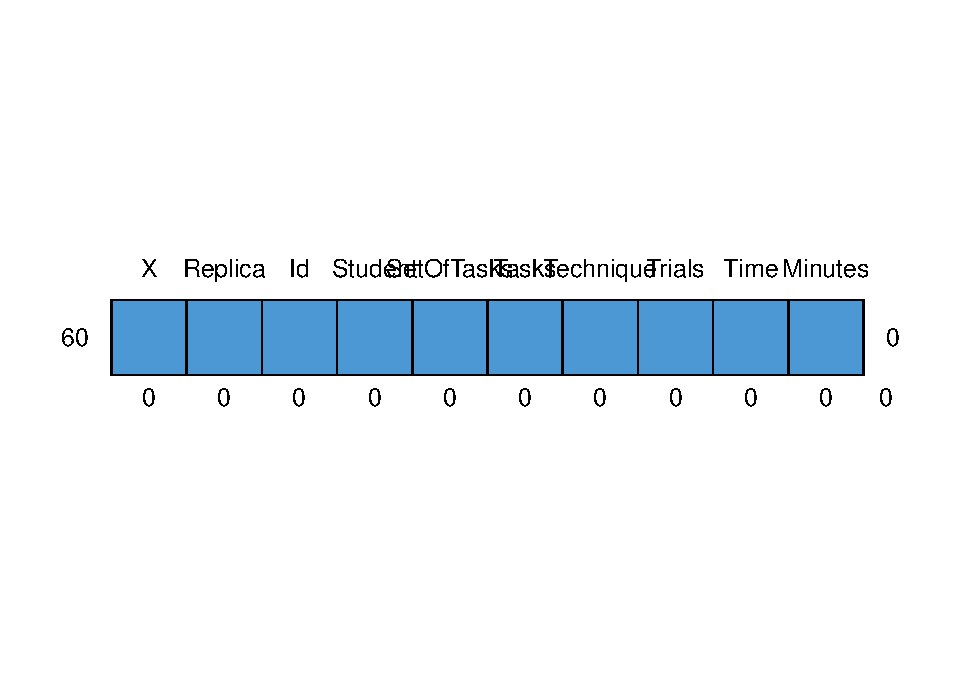
\includegraphics{main_files/figure-latex/unnamed-chunk-2-1.pdf}

\begin{verbatim}
##    X Replica Id Student SetOfTasks Tasks Technique Trials Time Minutes  
## 60 1       1  1       1          1     1         1      1    1       1 0
##    0       0  0       0          0     0         0      0    0       0 0
\end{verbatim}

\begin{verbatim}
## 
##  iter imp variable
##   1   1
##   1   2
##   1   3
##   1   4
##   1   5
##   2   1
##   2   2
##   2   3
##   2   4
##   2   5
##   3   1
##   3   2
##   3   3
##   3   4
##   3   5
##   4   1
##   4   2
##   4   3
##   4   4
##   4   5
##   5   1
##   5   2
##   5   3
##   5   4
##   5   5
##   6   1
##   6   2
##   6   3
##   6   4
##   6   5
##   7   1
##   7   2
##   7   3
##   7   4
##   7   5
##   8   1
##   8   2
##   8   3
##   8   4
##   8   5
##   9   1
##   9   2
##   9   3
##   9   4
##   9   5
##   10   1
##   10   2
##   10   3
##   10   4
##   10   5
##   11   1
##   11   2
##   11   3
##   11   4
##   11   5
##   12   1
##   12   2
##   12   3
##   12   4
##   12   5
##   13   1
##   13   2
##   13   3
##   13   4
##   13   5
##   14   1
##   14   2
##   14   3
##   14   4
##   14   5
##   15   1
##   15   2
##   15   3
##   15   4
##   15   5
##   16   1
##   16   2
##   16   3
##   16   4
##   16   5
##   17   1
##   17   2
##   17   3
##   17   4
##   17   5
##   18   1
##   18   2
##   18   3
##   18   4
##   18   5
##   19   1
##   19   2
##   19   3
##   19   4
##   19   5
##   20   1
##   20   2
##   20   3
##   20   4
##   20   5
##   21   1
##   21   2
##   21   3
##   21   4
##   21   5
##   22   1
##   22   2
##   22   3
##   22   4
##   22   5
##   23   1
##   23   2
##   23   3
##   23   4
##   23   5
##   24   1
##   24   2
##   24   3
##   24   4
##   24   5
##   25   1
##   25   2
##   25   3
##   25   4
##   25   5
##   26   1
##   26   2
##   26   3
##   26   4
##   26   5
##   27   1
##   27   2
##   27   3
##   27   4
##   27   5
##   28   1
##   28   2
##   28   3
##   28   4
##   28   5
##   29   1
##   29   2
##   29   3
##   29   4
##   29   5
##   30   1
##   30   2
##   30   3
##   30   4
##   30   5
##   31   1
##   31   2
##   31   3
##   31   4
##   31   5
##   32   1
##   32   2
##   32   3
##   32   4
##   32   5
##   33   1
##   33   2
##   33   3
##   33   4
##   33   5
##   34   1
##   34   2
##   34   3
##   34   4
##   34   5
##   35   1
##   35   2
##   35   3
##   35   4
##   35   5
##   36   1
##   36   2
##   36   3
##   36   4
##   36   5
##   37   1
##   37   2
##   37   3
##   37   4
##   37   5
##   38   1
##   38   2
##   38   3
##   38   4
##   38   5
##   39   1
##   39   2
##   39   3
##   39   4
##   39   5
##   40   1
##   40   2
##   40   3
##   40   4
##   40   5
##   41   1
##   41   2
##   41   3
##   41   4
##   41   5
##   42   1
##   42   2
##   42   3
##   42   4
##   42   5
##   43   1
##   43   2
##   43   3
##   43   4
##   43   5
##   44   1
##   44   2
##   44   3
##   44   4
##   44   5
##   45   1
##   45   2
##   45   3
##   45   4
##   45   5
##   46   1
##   46   2
##   46   3
##   46   4
##   46   5
##   47   1
##   47   2
##   47   3
##   47   4
##   47   5
##   48   1
##   48   2
##   48   3
##   48   4
##   48   5
##   49   1
##   49   2
##   49   3
##   49   4
##   49   5
##   50   1
##   50   2
##   50   3
##   50   4
##   50   5
\end{verbatim}

\begin{verbatim}
## Warning: Number of logged events: 1
\end{verbatim}

\begin{verbatim}
##    Replica Id SetOfTasks    Technique Trials Time
## 1       41  1        ST1 Without Atom      7   13
## 2       41  1        ST2    With Atom      3   16
## 3       41  2        ST1    With Atom      5   21
## 4       41  2        ST2 Without Atom      3   15
## 5       42  1        ST1 Without Atom      5   14
## 6       42  1        ST2    With Atom     12   39
## 7       42  2        ST1    With Atom      7   16
## 8       42  2        ST2 Without Atom     12   22
## 9       43  1        ST1 Without Atom      5   18
## 10      43  1        ST2    With Atom      9   53
## 11      43  2        ST1    With Atom      9   21
## 12      43  2        ST2 Without Atom      5   15
## 13      44  1        ST1 Without Atom      4    9
## 14      44  1        ST2    With Atom      4   24
## 15      44  2        ST1    With Atom      6   17
## 16      44  2        ST2 Without Atom      6   23
## 17      45  1        ST1    With Atom      9   25
## 18      45  1        ST2 Without Atom      7   28
## 19      45  2        ST1 Without Atom      5    7
## 20      45  2        ST2    With Atom      8   18
## 21      46  1        ST1    With Atom      7   32
## 22      46  1        ST2 Without Atom      9   32
## 23      46  2        ST1 Without Atom      4   10
## 24      46  2        ST2    With Atom     12   31
## 25      47  1        ST1 Without Atom      4   18
## 26      47  1        ST2    With Atom      5   53
## 27      47  2        ST1    With Atom      5   21
## 28      47  2        ST2 Without Atom      4   24
## 29      48  1        ST1    With Atom      7   15
## 30      48  1        ST2 Without Atom      3   12
## 31      48  2        ST1 Without Atom     10   25
## 32      48  2        ST2    With Atom     29   60
## 33      49  1        ST1 Without Atom      8   33
## 34      49  1        ST2    With Atom     10   23
## 35      49  2        ST1    With Atom      6    9
## 36      49  2        ST2 Without Atom      3    2
## 37      50  1        ST1    With Atom      8   21
## 38      50  1        ST2 Without Atom      5   19
## 39      50  2        ST1 Without Atom      7   19
## 40      50  2        ST2    With Atom     10   29
## 41      51  1        ST1 Without Atom      5   22
## 42      51  1        ST2    With Atom      6   24
## 43      51  2        ST1    With Atom      6    9
## 44      51  2        ST2 Without Atom      5   15
## 45      52  1        ST1    With Atom      9   23
## 46      52  1        ST2 Without Atom     24   38
## 47      52  2        ST1 Without Atom      7   16
## 48      52  2        ST2    With Atom     14   52
## 49      53  1        ST1    With Atom      5   11
## 50      53  1        ST2 Without Atom      4    8
## 51      53  2        ST1 Without Atom      5    9
## 52      53  2        ST2    With Atom     15   31
## 53      54  1        ST1 Without Atom      4   27
## 54      54  1        ST2    With Atom      7   34
## 55      54  2        ST1    With Atom      6   33
## 56      54  2        ST2 Without Atom      3   26
## 57      55  1        ST1    With Atom      5   23
## 58      55  1        ST2 Without Atom      4   19
## 59      55  2        ST1 Without Atom      5   10
## 60      55  2        ST2    With Atom     19   46
\end{verbatim}

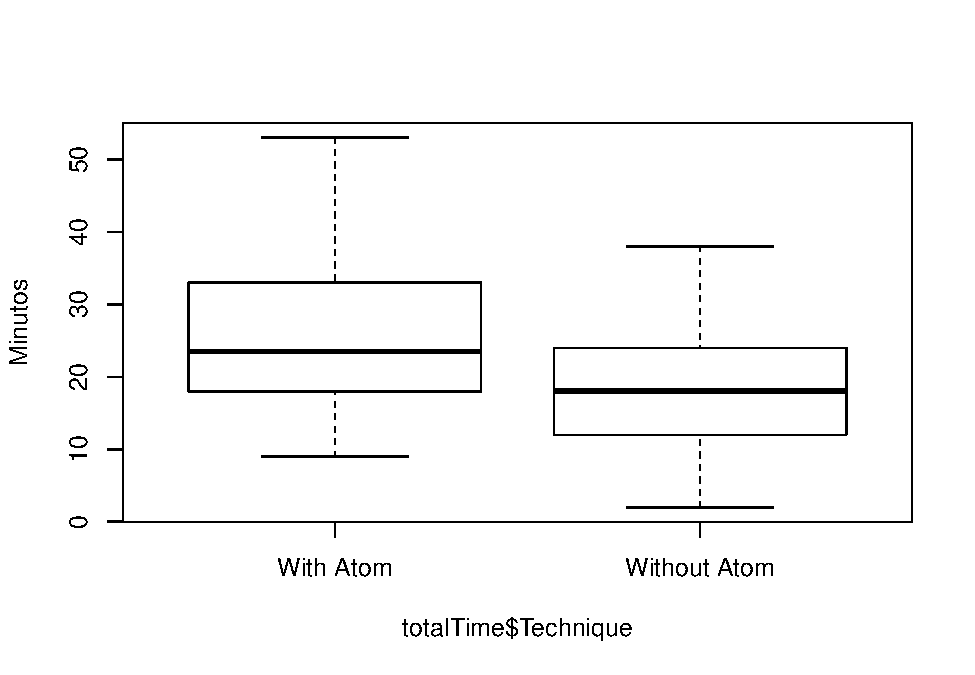
\includegraphics{main_files/figure-latex/unnamed-chunk-5-1.pdf}

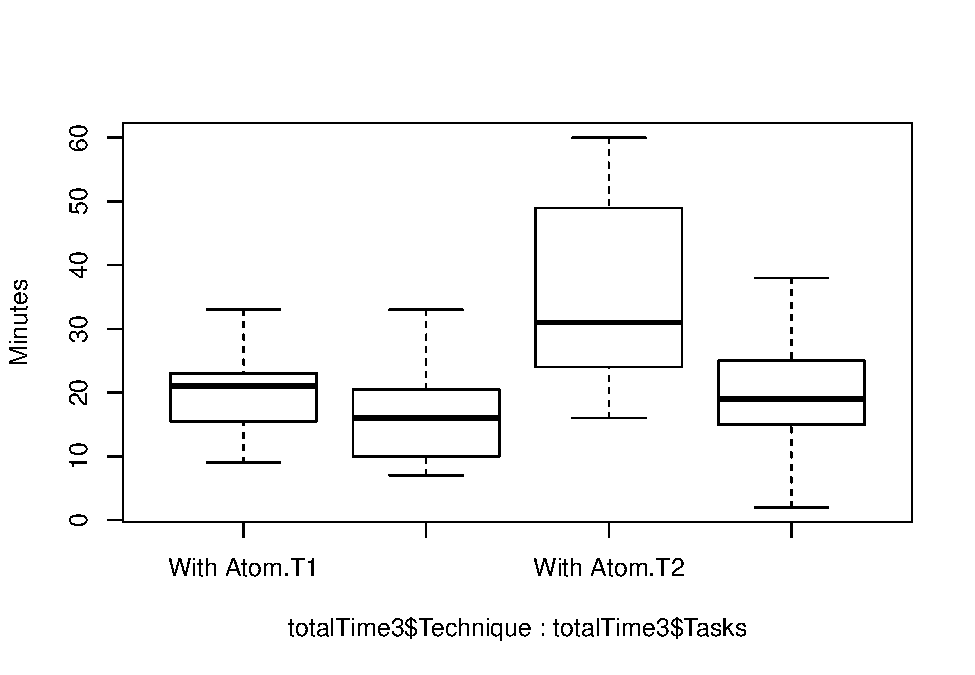
\includegraphics{main_files/figure-latex/unnamed-chunk-6-1.pdf}

\begin{verbatim}
##    Replica Tasks    Technique Trials Time
## 1       41    T1    With Atom      5   21
## 2       41    T1 Without Atom      7   13
## 3       41    T2    With Atom      3   16
## 4       41    T2 Without Atom      3   15
## 5       42    T1    With Atom      7   16
## 6       42    T1 Without Atom      5   14
## 7       42    T2    With Atom     12   39
## 8       42    T2 Without Atom     12   22
## 9       43    T1    With Atom      9   21
## 10      43    T1 Without Atom      5   18
## 11      43    T2    With Atom      9   53
## 12      43    T2 Without Atom      5   15
## 13      44    T1    With Atom      6   17
## 14      44    T1 Without Atom      4    9
## 15      44    T2    With Atom      4   24
## 16      44    T2 Without Atom      6   23
## 17      45    T1    With Atom      9   25
## 18      45    T1 Without Atom      5    7
## 19      45    T2    With Atom      8   18
## 20      45    T2 Without Atom      7   28
## 21      46    T1    With Atom      7   32
## 22      46    T1 Without Atom      4   10
## 23      46    T2    With Atom     12   31
## 24      46    T2 Without Atom      9   32
## 25      47    T1    With Atom      5   21
## 26      47    T1 Without Atom      4   18
## 27      47    T2    With Atom      5   53
## 28      47    T2 Without Atom      4   24
## 29      48    T1    With Atom      7   15
## 30      48    T1 Without Atom     10   25
## 31      48    T2    With Atom     29   60
## 32      48    T2 Without Atom      3   12
## 33      49    T1    With Atom      6    9
## 34      49    T1 Without Atom      8   33
## 35      49    T2    With Atom     10   23
## 36      49    T2 Without Atom      3    2
## 37      50    T1    With Atom      8   21
## 38      50    T1 Without Atom      7   19
## 39      50    T2    With Atom     10   29
## 40      50    T2 Without Atom      5   19
## 41      51    T1    With Atom      6    9
## 42      51    T1 Without Atom      5   22
## 43      51    T2    With Atom      6   24
## 44      51    T2 Without Atom      5   15
## 45      52    T1    With Atom      9   23
## 46      52    T1 Without Atom      7   16
## 47      52    T2    With Atom     14   52
## 48      52    T2 Without Atom     24   38
## 49      53    T1    With Atom      5   11
## 50      53    T1 Without Atom      5    9
## 51      53    T2    With Atom     15   31
## 52      53    T2 Without Atom      4    8
## 53      54    T1    With Atom      6   33
## 54      54    T1 Without Atom      4   27
## 55      54    T2    With Atom      7   34
## 56      54    T2 Without Atom      3   26
## 57      55    T1    With Atom      5   23
## 58      55    T1 Without Atom      5   10
## 59      55    T2    With Atom     19   46
## 60      55    T2 Without Atom      4   19
\end{verbatim}

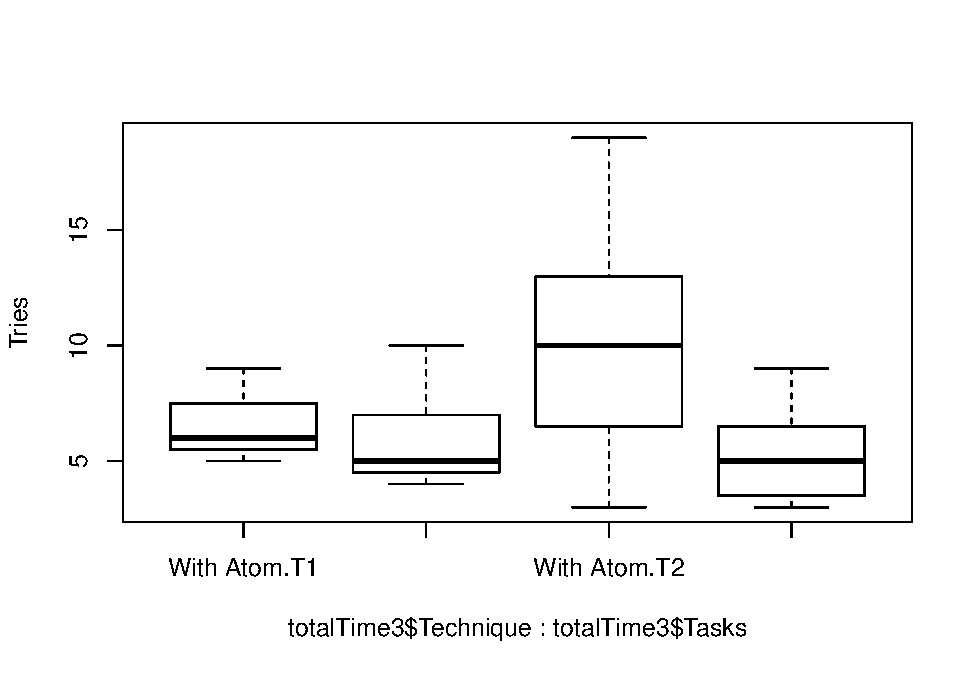
\includegraphics{main_files/figure-latex/unnamed-chunk-7-1.pdf}

\begin{verbatim}
##     X Replica Id                   Student SetOfTasks             Tasks
## 1   1      41  1                     paulo        ST1 AV1.2:CO1.2:DE1.2
## 2   1      41  1                     paulo        ST2 AV2.1:CO2.1:DE2.1
## 3   1      41  2                  Romário        ST1 AV1.1:CO1.1:DE1.1
## 4   1      41  2                  Romário        ST2 AV2.2:CO2.2:DE2.2
## 5   2      42  1                      Igor        ST1 AV1.2:CO1.2:DE1.2
## 6   2      42  1                      Igor        ST2 AV2.1:CO2.1:DE2.1
## 7   2      42  2                     Hyago        ST1 AV1.1:CO1.1:DE1.1
## 8   2      42  2                     Hyago        ST2 AV2.2:CO2.2:DE2.2
## 9   3      43  1                                  ST1 AV1.2:CO1.2:DE1.2
## 10  3      43  1                                  ST2 AV2.1:CO2.1:DE2.1
## 11  3      43  2                                  ST1 AV1.1:CO1.1:DE1.1
## 12  3      43  2                                  ST2 AV2.2:CO2.2:DE2.2
## 13  4      44  1                                  ST1 AV1.2:CO1.2:DE1.2
## 14  4      44  1                                  ST2 AV2.1:CO2.1:DE2.1
## 15  4      44  2                                  ST1 AV1.1:CO1.1:DE1.1
## 16  4      44  2                                  ST2 AV2.2:CO2.2:DE2.2
## 17  5      45  1             Matheus Costa        ST1 AV1.1:CO1.1:DE1.1
## 18  5      45  1             Matheus Costa        ST2 AV2.2:CO2.2:DE2.2
## 19  5      45  2                 Davi Jose        ST1 AV1.2:CO1.2:DE1.2
## 20  5      45  2                 Davi Jose        ST2 AV2.1:CO2.1:DE2.1
## 21  6      46  1             Marlon Lúcio        ST1 AV1.1:CO1.1:DE1.1
## 22  6      46  1             Marlon Lúcio        ST2 AV2.2:CO2.2:DE2.2
## 23  6      46  2  Jackson Barbosa da Silva        ST1 AV1.2:CO1.2:DE1.2
## 24  6      46  2  Jackson Barbosa da Silva        ST2 AV2.1:CO2.1:DE2.1
## 25  7      47  1                     Allan        ST1 AV1.2:CO1.2:DE1.2
## 26  7      47  1                     Allan        ST2 AV2.1:CO2.1:DE2.1
## 27  7      47  2 Dielson Sales de Carvalho        ST1 AV1.1:CO1.1:DE1.1
## 28  7      47  2 Dielson Sales de Carvalho        ST2 AV2.2:CO2.2:DE2.2
## 29  8      48  1                    Thiago        ST1 AV1.1:CO1.1:DE1.1
## 30  8      48  1                    Thiago        ST2 AV2.2:CO2.2:DE2.2
## 31  8      48  2                                  ST1 AV1.2:CO1.2:DE1.2
## 32  8      48  2                                  ST2 AV2.1:CO2.1:DE2.1
## 33  9      49  1              Rodrigo Lima        ST1 AV1.2:CO1.2:DE1.2
## 34  9      49  1              Rodrigo Lima        ST2 AV2.1:CO2.1:DE2.1
## 35  9      49  2              Jardel Costa        ST1 AV1.1:CO1.1:DE1.1
## 36  9      49  2              Jardel Costa        ST2 AV2.2:CO2.2:DE2.2
## 37 10      50  1             Felipe Pontes        ST1 AV1.1:CO1.1:DE1.1
## 38 10      50  1             Felipe Pontes        ST2 AV2.2:CO2.2:DE2.2
## 39 10      50  2               Jairo Souza        ST1 AV1.2:CO1.2:DE1.2
## 40 10      50  2               Jairo Souza        ST2 AV2.1:CO2.1:DE2.1
## 41 11      51  1                    julios        ST1 AV1.2:CO1.2:DE1.2
## 42 11      51  1                    julios        ST2 AV2.1:CO2.1:DE2.1
## 43 11      51  2          Romero Malaquias        ST1 AV1.1:CO1.1:DE1.1
## 44 11      51  2          Romero Malaquias        ST2 AV2.2:CO2.2:DE2.2
## 45 12      53  1 Bruno Georgevich Ferreira        ST1 AV1.1:CO1.1:DE1.1
## 46 12      53  1 Bruno Georgevich Ferreira        ST2 AV2.2:CO2.2:DE2.2
## 47 12      53  2                    jadson        ST1 AV1.2:CO1.2:DE1.2
## 48 12      53  2                    jadson        ST2 AV2.1:CO2.1:DE2.1
## 49 13      55  1                                  ST1 AV1.1:CO1.1:DE1.1
## 50 13      55  1                                  ST2 AV2.2:CO2.2:DE2.2
## 51 13      55  2                    Arthur        ST1 AV1.2:CO1.2:DE1.2
## 52 13      55  2                    Arthur        ST2 AV2.1:CO2.1:DE2.1
## 53 14      52  1                                  ST1 AV1.1:CO1.1:DE1.1
## 54 14      52  1                                  ST2 AV2.2:CO2.2:DE2.2
## 55 14      52  2            vinicius lopes        ST1 AV1.2:CO1.2:DE1.2
## 56 14      52  2            vinicius lopes        ST2 AV2.1:CO2.1:DE2.1
## 57 15      54  1            Thiago Tenorio        ST1 AV1.2:CO1.2:DE1.2
## 58 15      54  1            Thiago Tenorio        ST2 AV2.1:CO2.1:DE2.1
## 59 15      54  2 Joao Victor Ribeiro Ferro        ST1 AV1.1:CO1.1:DE1.1
## 60 15      54  2 Joao Victor Ribeiro Ferro        ST2 AV2.2:CO2.2:DE2.2
##       Technique Trials Time Minutes
## 1  Without Atom      7   13      13
## 2     With Atom      3   16      16
## 3     With Atom      5   21      21
## 4  Without Atom      3   15      15
## 5  Without Atom      5   14      14
## 6     With Atom     12   39      39
## 7     With Atom      7   16      16
## 8  Without Atom     12   22      22
## 9  Without Atom      5   18      18
## 10    With Atom      9   53      53
## 11    With Atom      9   21      21
## 12 Without Atom      5   15      15
## 13 Without Atom      4    9       9
## 14    With Atom      4   24      24
## 15    With Atom      6   17      17
## 16 Without Atom      6   23      23
## 17    With Atom      9   25      25
## 18 Without Atom      7   28      28
## 19 Without Atom      5    7       7
## 20    With Atom      8   18      18
## 21    With Atom      7   32      32
## 22 Without Atom      9   32      32
## 23 Without Atom      4   10      10
## 24    With Atom     12   31      31
## 25 Without Atom      4   18      18
## 26    With Atom      5   53      53
## 27    With Atom      5   21      21
## 28 Without Atom      4   24      24
## 29    With Atom      7   15      15
## 30 Without Atom      3   12      12
## 31 Without Atom     10   25      25
## 32    With Atom     29   60      60
## 33 Without Atom      8   33      33
## 34    With Atom     10   23      23
## 35    With Atom      6    9       9
## 36 Without Atom      3    2       2
## 37    With Atom      8   21      21
## 38 Without Atom      5   19      19
## 39 Without Atom      7   19      19
## 40    With Atom     10   29      29
## 41 Without Atom      5   22      22
## 42    With Atom      6   24      24
## 43    With Atom      6    9       9
## 44 Without Atom      5   15      15
## 45    With Atom      5   11      11
## 46 Without Atom      4    8       8
## 47 Without Atom      5    9       9
## 48    With Atom     15   31      31
## 49    With Atom      5   23      23
## 50 Without Atom      4   19      19
## 51 Without Atom      5   10      10
## 52    With Atom     19   46      46
## 53    With Atom      9   23      23
## 54 Without Atom     24   38      38
## 55 Without Atom      7   16      16
## 56    With Atom     14   52      52
## 57 Without Atom      4   27      27
## 58    With Atom      7   34      34
## 59    With Atom      6   33      33
## 60 Without Atom      3   26      26
\end{verbatim}

\begin{verbatim}
##    Replica             Tasks Minutes Time
## 1       41 AV1.2:CO1.2:DE1.2      13   13
## 2       41 AV1.1:CO1.1:DE1.1      21   21
## 3       42 AV1.2:CO1.2:DE1.2      14   14
## 4       42 AV1.1:CO1.1:DE1.1      16   16
## 5       43 AV1.2:CO1.2:DE1.2      18   18
## 6       43 AV1.1:CO1.1:DE1.1      21   21
## 7       44 AV1.2:CO1.2:DE1.2       9    9
## 8       44 AV1.1:CO1.1:DE1.1      17   17
## 9       45 AV1.1:CO1.1:DE1.1      25   25
## 10      45 AV1.2:CO1.2:DE1.2       7    7
## 11      46 AV1.1:CO1.1:DE1.1      32   32
## 12      46 AV1.2:CO1.2:DE1.2      10   10
## 13      47 AV1.2:CO1.2:DE1.2      18   18
## 14      47 AV1.1:CO1.1:DE1.1      21   21
## 15      48 AV1.1:CO1.1:DE1.1      15   15
## 16      48 AV1.2:CO1.2:DE1.2      25   25
## 17      49 AV1.2:CO1.2:DE1.2      33   33
## 18      49 AV1.1:CO1.1:DE1.1       9    9
## 19      50 AV1.1:CO1.1:DE1.1      21   21
## 20      50 AV1.2:CO1.2:DE1.2      19   19
## 21      51 AV1.2:CO1.2:DE1.2      22   22
## 22      51 AV1.1:CO1.1:DE1.1       9    9
## 23      53 AV1.1:CO1.1:DE1.1      11   11
## 24      53 AV1.2:CO1.2:DE1.2       9    9
## 25      55 AV1.1:CO1.1:DE1.1      23   23
## 26      55 AV1.2:CO1.2:DE1.2      10   10
## 27      52 AV1.1:CO1.1:DE1.1      23   23
## 28      52 AV1.2:CO1.2:DE1.2      16   16
## 29      54 AV1.2:CO1.2:DE1.2      27   27
## 30      54 AV1.1:CO1.1:DE1.1      33   33
\end{verbatim}

\begin{verbatim}
##    Replica             Tasks Minutes Time
## 1       41 AV2.1:CO2.1:DE2.1      16   16
## 2       41 AV2.2:CO2.2:DE2.2      15   15
## 3       42 AV2.1:CO2.1:DE2.1      39   39
## 4       42 AV2.2:CO2.2:DE2.2      22   22
## 5       43 AV2.1:CO2.1:DE2.1      53   53
## 6       43 AV2.2:CO2.2:DE2.2      15   15
## 7       44 AV2.1:CO2.1:DE2.1      24   24
## 8       44 AV2.2:CO2.2:DE2.2      23   23
## 9       45 AV2.2:CO2.2:DE2.2      28   28
## 10      45 AV2.1:CO2.1:DE2.1      18   18
## 11      46 AV2.2:CO2.2:DE2.2      32   32
## 12      46 AV2.1:CO2.1:DE2.1      31   31
## 13      47 AV2.1:CO2.1:DE2.1      53   53
## 14      47 AV2.2:CO2.2:DE2.2      24   24
## 15      48 AV2.2:CO2.2:DE2.2      12   12
## 16      48 AV2.1:CO2.1:DE2.1      60   60
## 17      49 AV2.1:CO2.1:DE2.1      23   23
## 18      49 AV2.2:CO2.2:DE2.2       2    2
## 19      50 AV2.2:CO2.2:DE2.2      19   19
## 20      50 AV2.1:CO2.1:DE2.1      29   29
## 21      51 AV2.1:CO2.1:DE2.1      24   24
## 22      51 AV2.2:CO2.2:DE2.2      15   15
## 23      53 AV2.2:CO2.2:DE2.2       8    8
## 24      53 AV2.1:CO2.1:DE2.1      31   31
## 25      55 AV2.2:CO2.2:DE2.2      19   19
## 26      55 AV2.1:CO2.1:DE2.1      46   46
## 27      52 AV2.2:CO2.2:DE2.2      38   38
## 28      52 AV2.1:CO2.1:DE2.1      52   52
## 29      54 AV2.1:CO2.1:DE2.1      34   34
## 30      54 AV2.2:CO2.2:DE2.2      26   26
\end{verbatim}

\begin{verbatim}
## [1] 18.23333
\end{verbatim}

\begin{verbatim}
## [1] 27.7
\end{verbatim}

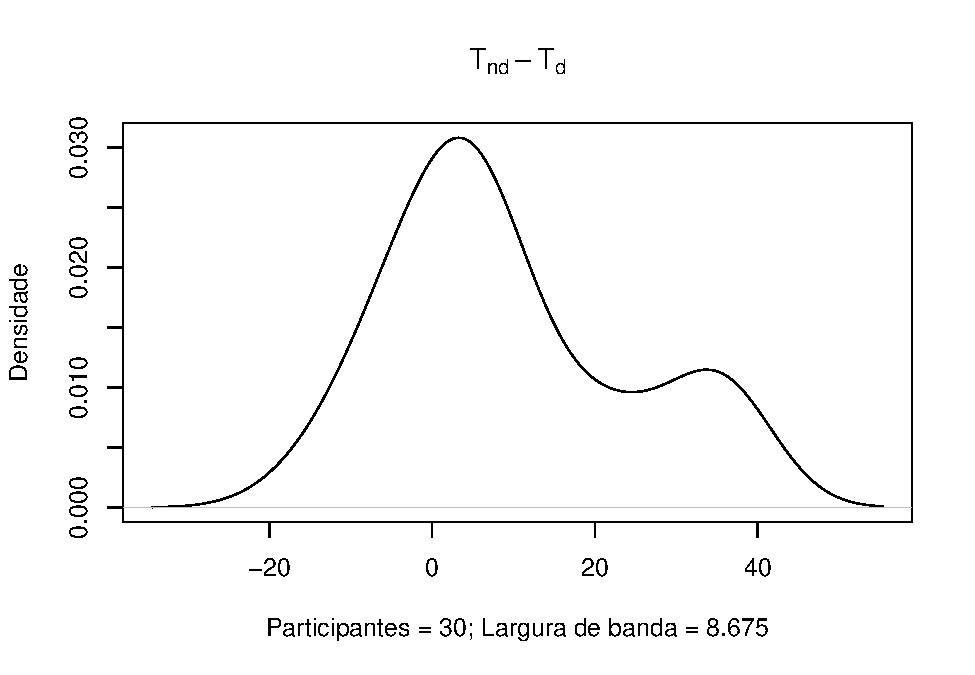
\includegraphics{main_files/figure-latex/unnamed-chunk-8-1.pdf}

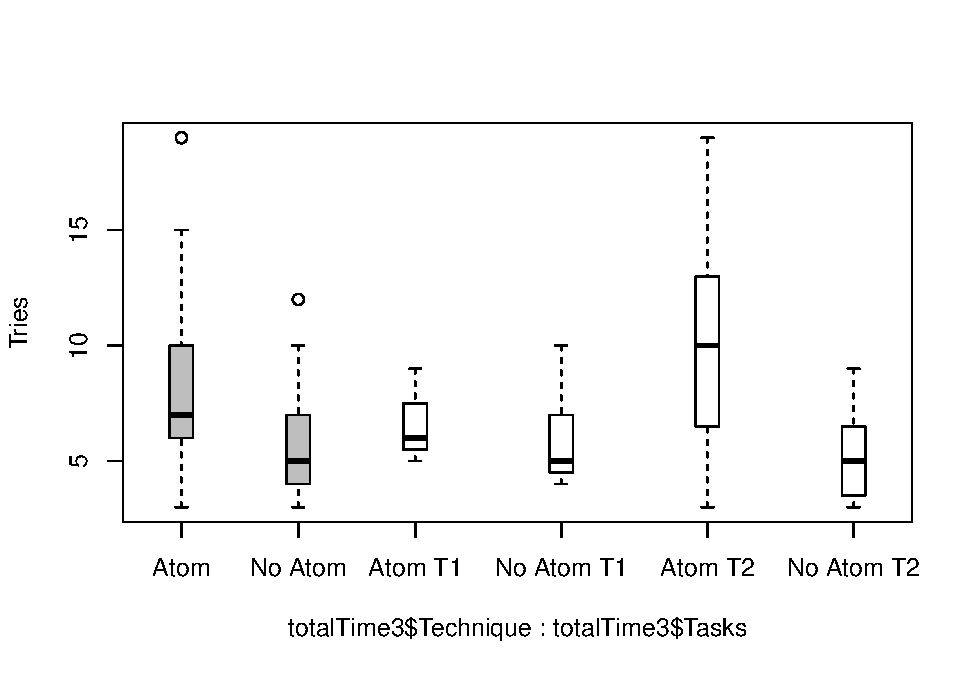
\includegraphics{main_files/figure-latex/unnamed-chunk-9-1.pdf}

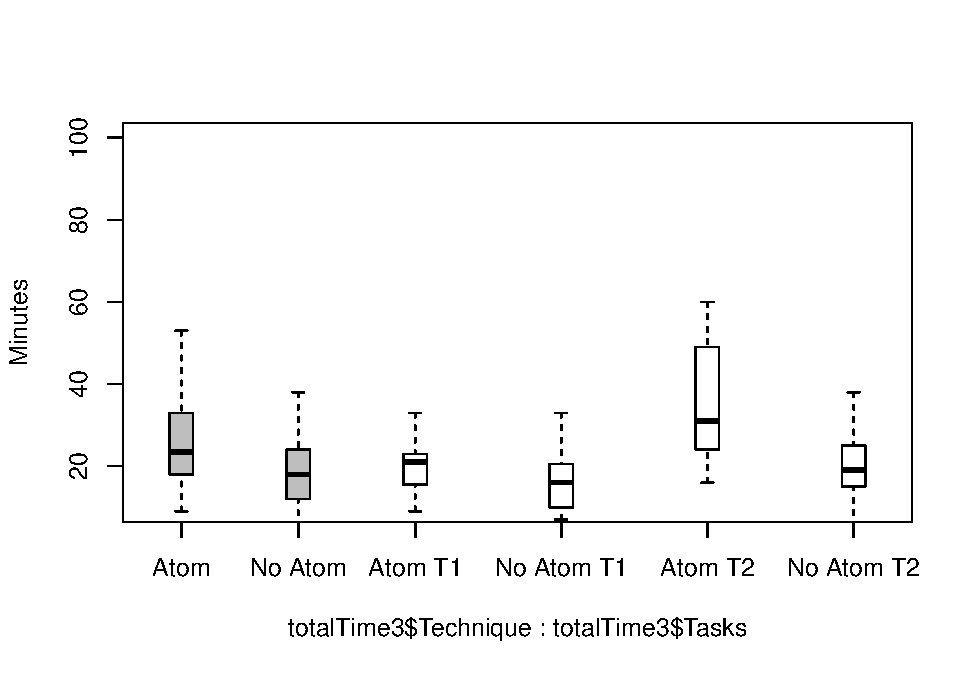
\includegraphics{main_files/figure-latex/unnamed-chunk-10-1.pdf}

\begin{Shaded}
\begin{Highlighting}[]
\NormalTok{totalTrials <-}\StringTok{ }\KeywordTok{sqldf}\NormalTok{(}\StringTok{"select Replica, Id, SetOfTasks,}
\StringTok{                      Technique, sum(Trials) as Trials}
\StringTok{                      from ccwocd}
\StringTok{                      group by Replica, Id,SetOfTasks, Technique"}\NormalTok{)}

\NormalTok{totalTrials}
\end{Highlighting}
\end{Shaded}

\begin{verbatim}
##    Replica Id SetOfTasks    Technique Trials
## 1       41  1        ST1 Without Atom      7
## 2       41  1        ST2    With Atom      3
## 3       41  2        ST1    With Atom      5
## 4       41  2        ST2 Without Atom      3
## 5       42  1        ST1 Without Atom      5
## 6       42  1        ST2    With Atom     12
## 7       42  2        ST1    With Atom      7
## 8       42  2        ST2 Without Atom     12
## 9       43  1        ST1 Without Atom      5
## 10      43  1        ST2    With Atom      9
## 11      43  2        ST1    With Atom      9
## 12      43  2        ST2 Without Atom      5
## 13      44  1        ST1 Without Atom      4
## 14      44  1        ST2    With Atom      4
## 15      44  2        ST1    With Atom      6
## 16      44  2        ST2 Without Atom      6
## 17      45  1        ST1    With Atom      9
## 18      45  1        ST2 Without Atom      7
## 19      45  2        ST1 Without Atom      5
## 20      45  2        ST2    With Atom      8
## 21      46  1        ST1    With Atom      7
## 22      46  1        ST2 Without Atom      9
## 23      46  2        ST1 Without Atom      4
## 24      46  2        ST2    With Atom     12
## 25      47  1        ST1 Without Atom      4
## 26      47  1        ST2    With Atom      5
## 27      47  2        ST1    With Atom      5
## 28      47  2        ST2 Without Atom      4
## 29      48  1        ST1    With Atom      7
## 30      48  1        ST2 Without Atom      3
## 31      48  2        ST1 Without Atom     10
## 32      48  2        ST2    With Atom     29
## 33      49  1        ST1 Without Atom      8
## 34      49  1        ST2    With Atom     10
## 35      49  2        ST1    With Atom      6
## 36      49  2        ST2 Without Atom      3
## 37      50  1        ST1    With Atom      8
## 38      50  1        ST2 Without Atom      5
## 39      50  2        ST1 Without Atom      7
## 40      50  2        ST2    With Atom     10
## 41      51  1        ST1 Without Atom      5
## 42      51  1        ST2    With Atom      6
## 43      51  2        ST1    With Atom      6
## 44      51  2        ST2 Without Atom      5
## 45      52  1        ST1    With Atom      9
## 46      52  1        ST2 Without Atom     24
## 47      52  2        ST1 Without Atom      7
## 48      52  2        ST2    With Atom     14
## 49      53  1        ST1    With Atom      5
## 50      53  1        ST2 Without Atom      4
## 51      53  2        ST1 Without Atom      5
## 52      53  2        ST2    With Atom     15
## 53      54  1        ST1 Without Atom      4
## 54      54  1        ST2    With Atom      7
## 55      54  2        ST1    With Atom      6
## 56      54  2        ST2 Without Atom      3
## 57      55  1        ST1    With Atom      5
## 58      55  1        ST2 Without Atom      4
## 59      55  2        ST1 Without Atom      5
## 60      55  2        ST2    With Atom     19
\end{verbatim}

\begin{Shaded}
\begin{Highlighting}[]
\KeywordTok{boxplot}\NormalTok{(totalTrials}\OperatorTok{$}\NormalTok{Trials}\OperatorTok{~}\NormalTok{totalTrials}\OperatorTok{$}\NormalTok{Technique, }
        \CommentTok{#names=c("Disciplinado", "Não disciplinado")}
        \CommentTok{#names=c("Disciplined", "Undisciplined")}
\NormalTok{        )}
\end{Highlighting}
\end{Shaded}

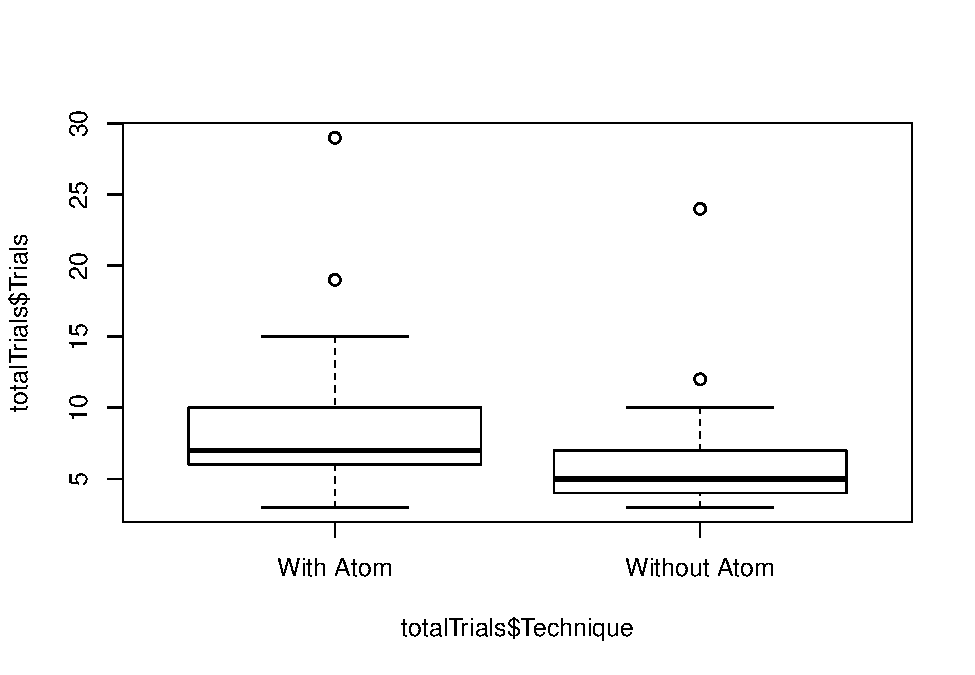
\includegraphics{main_files/figure-latex/unnamed-chunk-11-1.pdf}

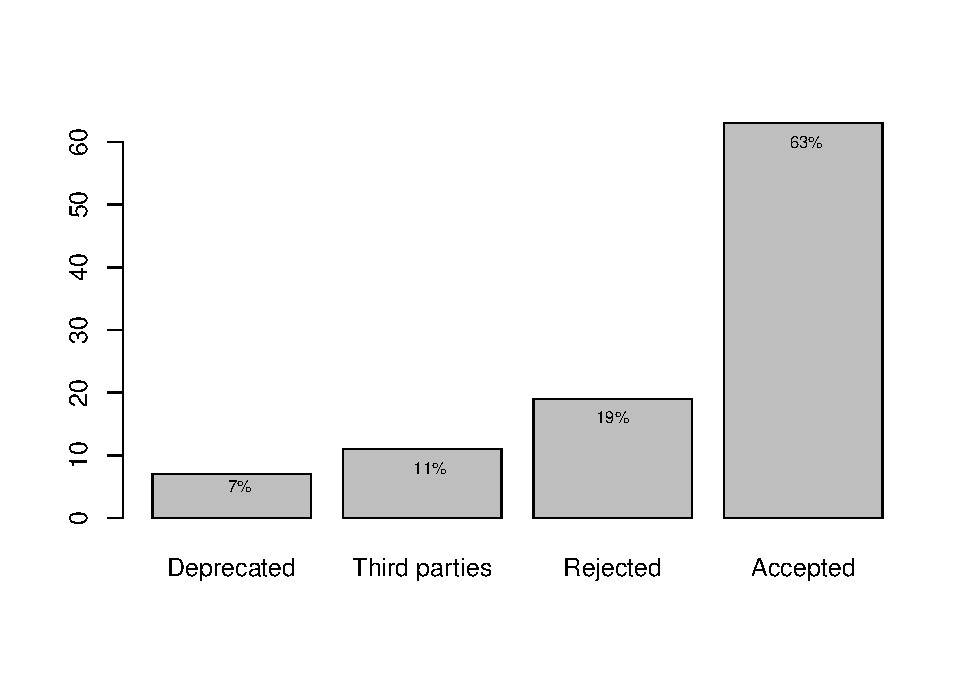
\includegraphics{main_files/figure-latex/unnamed-chunk-12-1.pdf}

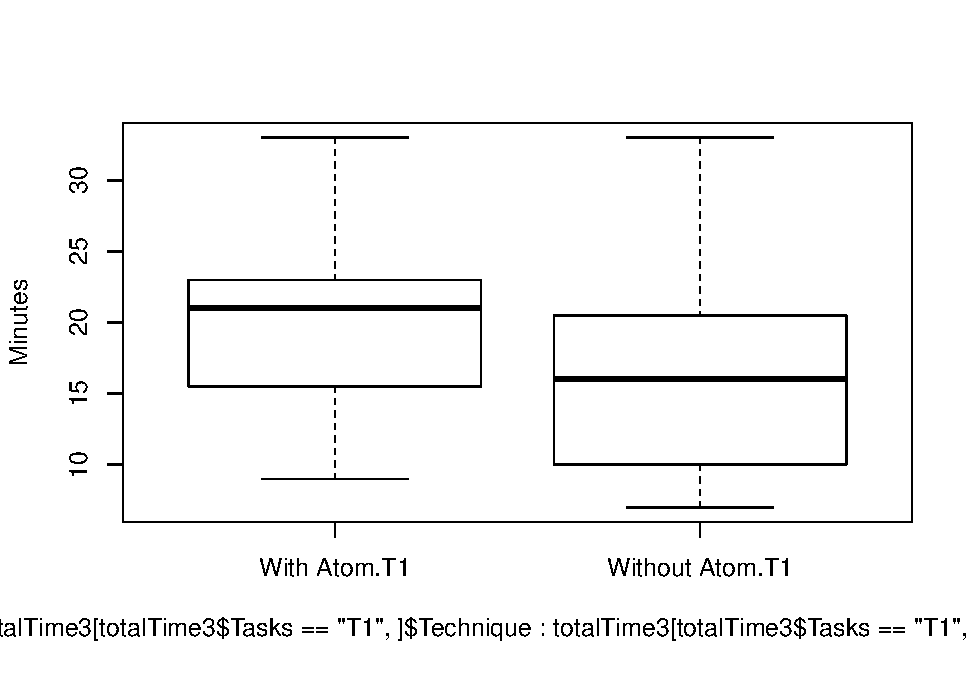
\includegraphics{main_files/figure-latex/unnamed-chunk-13-1.pdf}
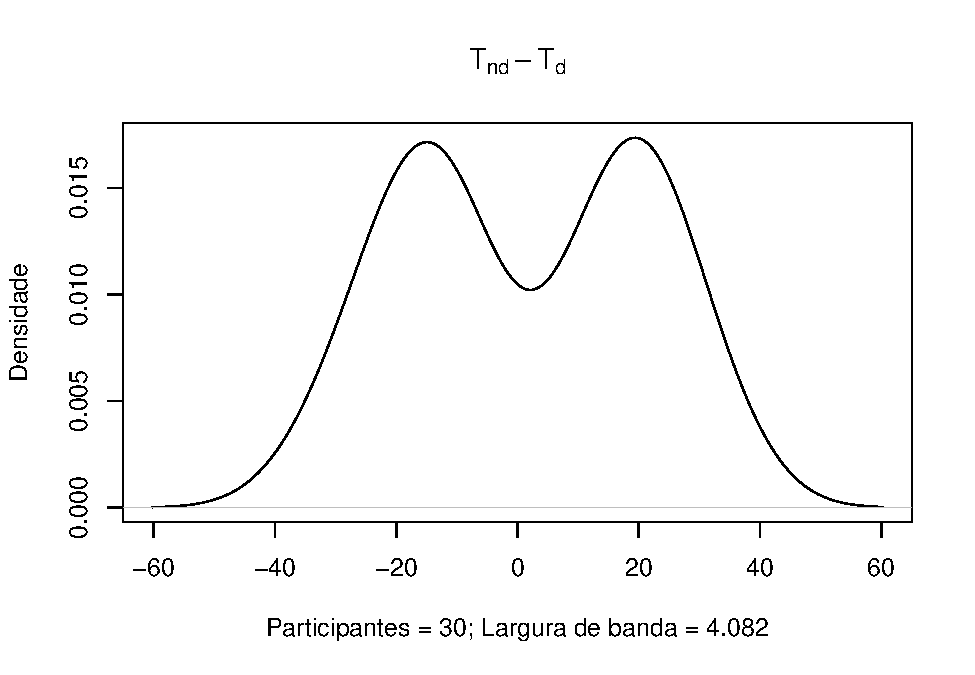
\includegraphics{main_files/figure-latex/unnamed-chunk-14-1.pdf}

\begin{Shaded}
\begin{Highlighting}[]
\NormalTok{totalTime <-}\StringTok{ }\KeywordTok{sqldf}\NormalTok{(}\StringTok{"select Replica, Id, SetOfTasks, }
\StringTok{                    Technique, sum(Trials) as Trials, sum(Minutes) as Time }
\StringTok{                    from ccwocd where Tasks = 'AV1.1:CO1.1:DE1.1' or Tasks = 'AV1.2:CO1.2:DE1.2'}
\StringTok{                    group by Replica, Id,SetOfTasks, Technique"}\NormalTok{)}




\CommentTok{#totalTime$Trials <- with(totalTime, (Trials - min(Trials)) / (max(Trials) - min(Trials)))}
\CommentTok{#totalTime$Time <- with(totalTime, (Time - min(Time)) / (max(Time) - min(Time)))}
\CommentTok{#totalTime$Trials <- with(totalTime, sqrt(Trials))}
\CommentTok{#totalTime$Time <- with(totalTime, sqrt(Time))}
\NormalTok{totalTime}\OperatorTok{$}\NormalTok{Time <-}\StringTok{ }\KeywordTok{with}\NormalTok{(totalTime, }\KeywordTok{log2}\NormalTok{(Time))}
\end{Highlighting}
\end{Shaded}

\begin{Shaded}
\begin{Highlighting}[]
\NormalTok{totalTime}\OperatorTok{$}\NormalTok{Replica =}\StringTok{ }\KeywordTok{as.factor}\NormalTok{(totalTime}\OperatorTok{$}\NormalTok{Replica)}
\NormalTok{totalTime}\OperatorTok{$}\NormalTok{Id =}\StringTok{ }\KeywordTok{as.factor}\NormalTok{(totalTime}\OperatorTok{$}\NormalTok{Id)}
\NormalTok{totalTime}\OperatorTok{$}\NormalTok{SetOfTasks =}\StringTok{ }\KeywordTok{as.factor}\NormalTok{(totalTime}\OperatorTok{$}\NormalTok{SetOfTasks)}
\NormalTok{totalTime}\OperatorTok{$}\NormalTok{Technique =}\StringTok{ }\KeywordTok{as.factor}\NormalTok{(totalTime}\OperatorTok{$}\NormalTok{Technique)}
\end{Highlighting}
\end{Shaded}

\begin{Shaded}
\begin{Highlighting}[]
\NormalTok{totalTime.gvlma =}\StringTok{ }\KeywordTok{gvlma}\NormalTok{(}\KeywordTok{lm}\NormalTok{(Time }\OperatorTok{~}\StringTok{ }\NormalTok{Technique, }\DataTypeTok{data=}\NormalTok{totalTime))}
\KeywordTok{summary}\NormalTok{(totalTime.gvlma)}
\end{Highlighting}
\end{Shaded}

\begin{verbatim}
## 
## Call:
## lm(formula = Time ~ Technique, data = totalTime)
## 
## Residuals:
##     Min      1Q  Median      3Q     Max 
## -1.1119 -0.5229  0.1858  0.3257  1.1251 
## 
## Coefficients:
##                       Estimate Std. Error t value Pr(>|t|)    
## (Intercept)             4.2066     0.1609  26.147   <2e-16 ***
## TechniqueWithout Atom  -0.2873     0.2275  -1.263    0.217    
## ---
## Signif. codes:  0 '***' 0.001 '**' 0.01 '*' 0.05 '.' 0.1 ' ' 1
## 
## Residual standard error: 0.6231 on 28 degrees of freedom
## Multiple R-squared:  0.05387,    Adjusted R-squared:  0.02008 
## F-statistic: 1.594 on 1 and 28 DF,  p-value: 0.2171
## 
## 
## ASSESSMENT OF THE LINEAR MODEL ASSUMPTIONS
## USING THE GLOBAL TEST ON 4 DEGREES-OF-FREEDOM:
## Level of Significance =  0.05 
## 
## Call:
##  gvlma(x = lm(Time ~ Technique, data = totalTime)) 
## 
##                        Value p-value                Decision
## Global Stat        2.611e+00  0.6249 Assumptions acceptable.
## Skewness           2.499e-01  0.6171 Assumptions acceptable.
## Kurtosis           9.031e-01  0.3419 Assumptions acceptable.
## Link Function      1.105e-15  1.0000 Assumptions acceptable.
## Heteroscedasticity 1.458e+00  0.2272 Assumptions acceptable.
\end{verbatim}

\begin{Shaded}
\begin{Highlighting}[]
\KeywordTok{summary}\NormalTok{(}\KeywordTok{aov}\NormalTok{(}\KeywordTok{lm}\NormalTok{(Time }\OperatorTok{~}\StringTok{ }\NormalTok{Technique, }\DataTypeTok{data=}\NormalTok{totalTime)))}
\end{Highlighting}
\end{Shaded}

\begin{verbatim}
##             Df Sum Sq Mean Sq F value Pr(>F)
## Technique    1  0.619  0.6189   1.594  0.217
## Residuals   28 10.870  0.3882
\end{verbatim}

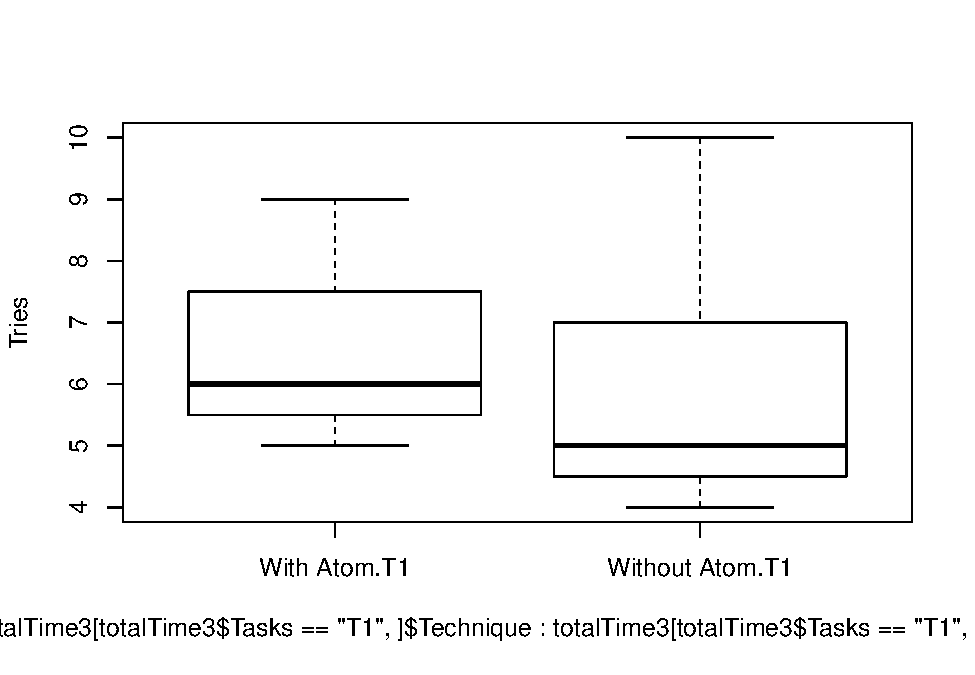
\includegraphics{main_files/figure-latex/unnamed-chunk-19-1.pdf}

\begin{Shaded}
\begin{Highlighting}[]
\NormalTok{totalTrials <-}\StringTok{ }\KeywordTok{sqldf}\NormalTok{(}\StringTok{"select Replica, Id, SetOfTasks,}
\StringTok{                      Technique, sum(Trials) as Trials}
\StringTok{                      from ccwocd where Tasks = 'AV1.1:CO1.1:DE1.1' or Tasks = 'AV1.2:CO1.2:DE1.2'}
\StringTok{                      group by Replica, Id,SetOfTasks, Technique"}\NormalTok{)}
\NormalTok{totalTrials}\OperatorTok{$}\NormalTok{Trials <-}\StringTok{ }\KeywordTok{with}\NormalTok{(totalTrials, Trials }\OperatorTok{+}\StringTok{ }\DecValTok{1}\NormalTok{)}
\NormalTok{totalTrials}\OperatorTok{$}\NormalTok{Trials <-}\StringTok{ }\KeywordTok{with}\NormalTok{(totalTrials, }\KeywordTok{log2}\NormalTok{(Trials))}
\end{Highlighting}
\end{Shaded}

\begin{Shaded}
\begin{Highlighting}[]
\NormalTok{totalTrials}\OperatorTok{$}\NormalTok{Replica =}\StringTok{ }\KeywordTok{as.factor}\NormalTok{(totalTrials}\OperatorTok{$}\NormalTok{Replica)}
\NormalTok{totalTrials}\OperatorTok{$}\NormalTok{Id =}\StringTok{ }\KeywordTok{as.factor}\NormalTok{(totalTrials}\OperatorTok{$}\NormalTok{Id)}
\NormalTok{totalTrials}\OperatorTok{$}\NormalTok{SetOfTasks =}\StringTok{ }\KeywordTok{as.factor}\NormalTok{(totalTrials}\OperatorTok{$}\NormalTok{SetOfTasks}\OperatorTok{:}\NormalTok{totalTrials}\OperatorTok{$}\NormalTok{Technique)}
\NormalTok{totalTrials}\OperatorTok{$}\NormalTok{Technique =}\StringTok{ }\KeywordTok{as.factor}\NormalTok{(totalTrials}\OperatorTok{$}\NormalTok{Technique)}
\end{Highlighting}
\end{Shaded}

\begin{Shaded}
\begin{Highlighting}[]
\KeywordTok{summary}\NormalTok{(}\KeywordTok{aov}\NormalTok{(Trials }\OperatorTok{~}\StringTok{ }\NormalTok{Replica }\OperatorTok{+}\StringTok{ }\NormalTok{Replica}\OperatorTok{:}\NormalTok{Id }\OperatorTok{+}\StringTok{ }\NormalTok{SetOfTasks }\OperatorTok{+}\StringTok{ }\NormalTok{Technique, }\DataTypeTok{data=}\NormalTok{totalTrials))}
\end{Highlighting}
\end{Shaded}

\begin{verbatim}
##             Df Sum Sq Mean Sq
## Replica     14 1.6643  0.1189
## SetOfTasks   1 0.3582  0.3582
## Replica:Id  14 1.1195  0.0800
\end{verbatim}

\begin{Shaded}
\begin{Highlighting}[]
\NormalTok{totalTrials.gvlma =}\StringTok{ }\KeywordTok{gvlma}\NormalTok{(}\KeywordTok{lm}\NormalTok{(Trials }\OperatorTok{~}\StringTok{ }\NormalTok{Technique, }\DataTypeTok{data=}\NormalTok{totalTrials))}
\KeywordTok{summary}\NormalTok{(totalTrials.gvlma)}
\end{Highlighting}
\end{Shaded}

\begin{verbatim}
## 
## Call:
## lm(formula = Trials ~ Technique, data = totalTrials)
## 
## Residuals:
##     Min      1Q  Median      3Q     Max 
## -0.3732 -0.2741 -0.1063  0.2927  0.7643 
## 
## Coefficients:
##                       Estimate Std. Error t value Pr(>|t|)    
## (Intercept)            2.91367    0.08141  35.789   <2e-16 ***
## TechniqueWithout Atom -0.21854    0.11514  -1.898    0.068 .  
## ---
## Signif. codes:  0 '***' 0.001 '**' 0.01 '*' 0.05 '.' 0.1 ' ' 1
## 
## Residual standard error: 0.3153 on 28 degrees of freedom
## Multiple R-squared:  0.114,  Adjusted R-squared:  0.08236 
## F-statistic: 3.603 on 1 and 28 DF,  p-value: 0.06803
## 
## 
## ASSESSMENT OF THE LINEAR MODEL ASSUMPTIONS
## USING THE GLOBAL TEST ON 4 DEGREES-OF-FREEDOM:
## Level of Significance =  0.05 
## 
## Call:
##  gvlma(x = lm(Trials ~ Technique, data = totalTrials)) 
## 
##                         Value p-value                Decision
## Global Stat        -3.799e+01  1.0000 Assumptions acceptable.
## Skewness            1.729e+00  0.1886 Assumptions acceptable.
## Kurtosis            3.856e-01  0.5346 Assumptions acceptable.
## Link Function      -4.011e+01  1.0000 Assumptions acceptable.
## Heteroscedasticity  9.333e-04  0.9756 Assumptions acceptable.
\end{verbatim}

\begin{Shaded}
\begin{Highlighting}[]
\KeywordTok{summary}\NormalTok{(}\KeywordTok{aov}\NormalTok{(Trials }\OperatorTok{~}\StringTok{ }\NormalTok{Technique, }\DataTypeTok{data=}\NormalTok{totalTrials))}
\end{Highlighting}
\end{Shaded}

\begin{verbatim}
##             Df Sum Sq Mean Sq F value Pr(>F)  
## Technique    1 0.3582  0.3582   3.603  0.068 .
## Residuals   28 2.7838  0.0994                 
## ---
## Signif. codes:  0 '***' 0.001 '**' 0.01 '*' 0.05 '.' 0.1 ' ' 1
\end{verbatim}

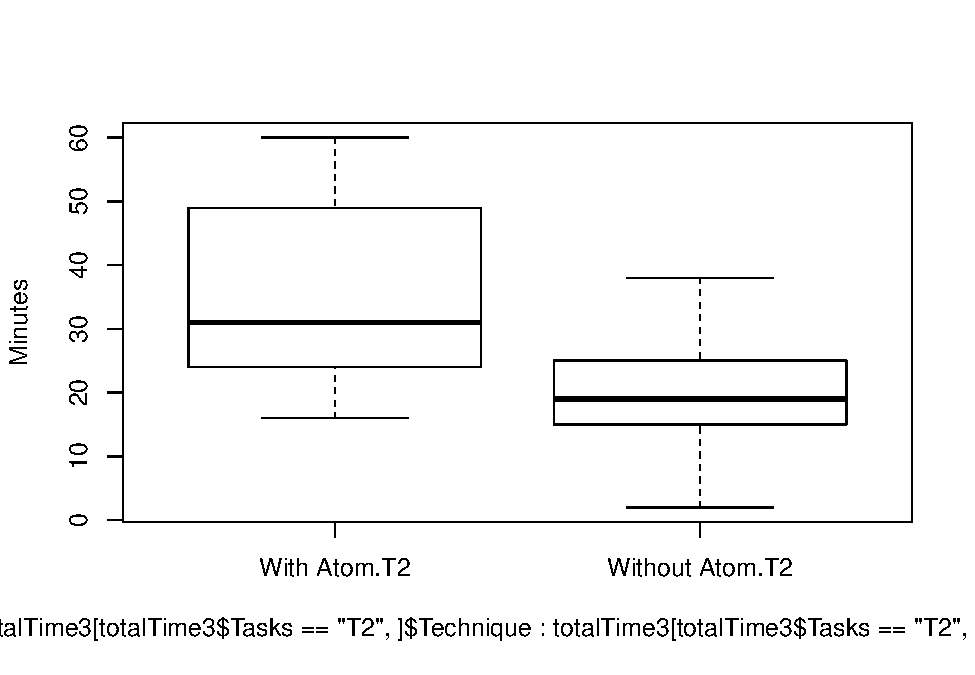
\includegraphics{main_files/figure-latex/unnamed-chunk-24-1.pdf}
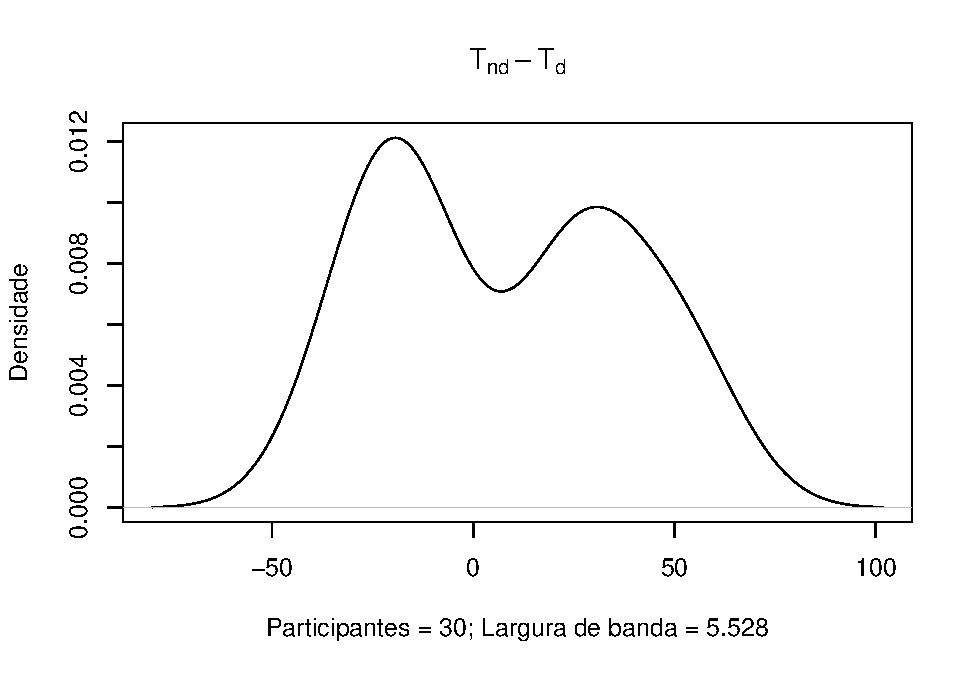
\includegraphics{main_files/figure-latex/unnamed-chunk-25-1.pdf}

\begin{Shaded}
\begin{Highlighting}[]
\NormalTok{totalTime <-}\StringTok{ }\KeywordTok{sqldf}\NormalTok{(}\StringTok{"select Replica, Id, SetOfTasks, }
\StringTok{                    Technique, sum(Trials) as Trials, sum(Minutes) as Time }
\StringTok{                    from ccwocd where Tasks = 'AV2.1:CO2.1:DE2.1' or Tasks = 'AV2.2:CO2.2:DE2.2'}
\StringTok{                    group by Replica, Id,SetOfTasks, Technique"}\NormalTok{)}

\NormalTok{totalTime}\OperatorTok{$}\NormalTok{Time <-}\StringTok{ }\KeywordTok{with}\NormalTok{(totalTime, }\KeywordTok{log2}\NormalTok{(Time))}
\end{Highlighting}
\end{Shaded}

\begin{Shaded}
\begin{Highlighting}[]
\NormalTok{totalTime}\OperatorTok{$}\NormalTok{Replica =}\StringTok{ }\KeywordTok{as.factor}\NormalTok{(totalTime}\OperatorTok{$}\NormalTok{Replica)}
\NormalTok{totalTime}\OperatorTok{$}\NormalTok{Id =}\StringTok{ }\KeywordTok{as.factor}\NormalTok{(totalTime}\OperatorTok{$}\NormalTok{Id)}
\NormalTok{totalTime}\OperatorTok{$}\NormalTok{SetOfTasks =}\StringTok{ }\KeywordTok{as.factor}\NormalTok{(totalTime}\OperatorTok{$}\NormalTok{SetOfTasks}\OperatorTok{:}\NormalTok{totalTime}\OperatorTok{$}\NormalTok{Id)}
\NormalTok{totalTime}\OperatorTok{$}\NormalTok{Technique =}\StringTok{ }\KeywordTok{as.factor}\NormalTok{(totalTime}\OperatorTok{$}\NormalTok{Technique)}
\end{Highlighting}
\end{Shaded}

\begin{Shaded}
\begin{Highlighting}[]
\NormalTok{totalTime.gvlma =}\StringTok{ }\KeywordTok{gvlma}\NormalTok{(}\KeywordTok{lm}\NormalTok{(Time }\OperatorTok{~}\StringTok{ }\NormalTok{Technique }\OperatorTok{+}\StringTok{ }\NormalTok{SetOfTasks, }\DataTypeTok{data=}\NormalTok{totalTime))}
\KeywordTok{summary}\NormalTok{(totalTime.gvlma)}
\end{Highlighting}
\end{Shaded}

\begin{verbatim}
## 
## Call:
## lm(formula = Time ~ Technique + SetOfTasks, data = totalTime)
## 
## Residuals:
##      Min       1Q   Median       3Q      Max 
## -3.02383 -0.40984  0.05571  0.61837  1.11443 
## 
## Coefficients:
##                       Estimate Std. Error t value Pr(>|t|)    
## (Intercept)             5.0905     0.2642  19.265  < 2e-16 ***
## TechniqueWithout Atom  -0.9570     0.3124  -3.064  0.00491 ** 
## SetOfTasksST2:2        -0.1097     0.3124  -0.351  0.72825    
## ---
## Signif. codes:  0 '***' 0.001 '**' 0.01 '*' 0.05 '.' 0.1 ' ' 1
## 
## Residual standard error: 0.8536 on 27 degrees of freedom
## Multiple R-squared:  0.2642, Adjusted R-squared:  0.2097 
## F-statistic: 4.847 on 2 and 27 DF,  p-value: 0.01589
## 
## 
## ASSESSMENT OF THE LINEAR MODEL ASSUMPTIONS
## USING THE GLOBAL TEST ON 4 DEGREES-OF-FREEDOM:
## Level of Significance =  0.05 
## 
## Call:
##  gvlma(x = lm(Time ~ Technique + SetOfTasks, data = totalTime)) 
## 
##                      Value   p-value                   Decision
## Global Stat        36.4165 2.375e-07 Assumptions NOT satisfied!
## Skewness           14.0019 1.826e-04 Assumptions NOT satisfied!
## Kurtosis           20.9989 4.595e-06 Assumptions NOT satisfied!
## Link Function       1.1795 2.774e-01    Assumptions acceptable.
## Heteroscedasticity  0.2362 6.270e-01    Assumptions acceptable.
\end{verbatim}

\begin{Shaded}
\begin{Highlighting}[]
\KeywordTok{summary}\NormalTok{(}\KeywordTok{aov}\NormalTok{(}\KeywordTok{lm}\NormalTok{(Time }\OperatorTok{~}\StringTok{ }\NormalTok{Technique, }\DataTypeTok{data=}\NormalTok{totalTime)))}
\end{Highlighting}
\end{Shaded}

\begin{verbatim}
##             Df Sum Sq Mean Sq F value  Pr(>F)   
## Technique    1  6.974   6.974   9.881 0.00393 **
## Residuals   28 19.762   0.706                   
## ---
## Signif. codes:  0 '***' 0.001 '**' 0.01 '*' 0.05 '.' 0.1 ' ' 1
\end{verbatim}

\begin{verbatim}
## 
##  Kruskal-Wallis rank sum test
## 
## data:  Time by Technique
## Kruskal-Wallis chi-squared = 9.1927, df = 1, p-value = 0.00243
\end{verbatim}

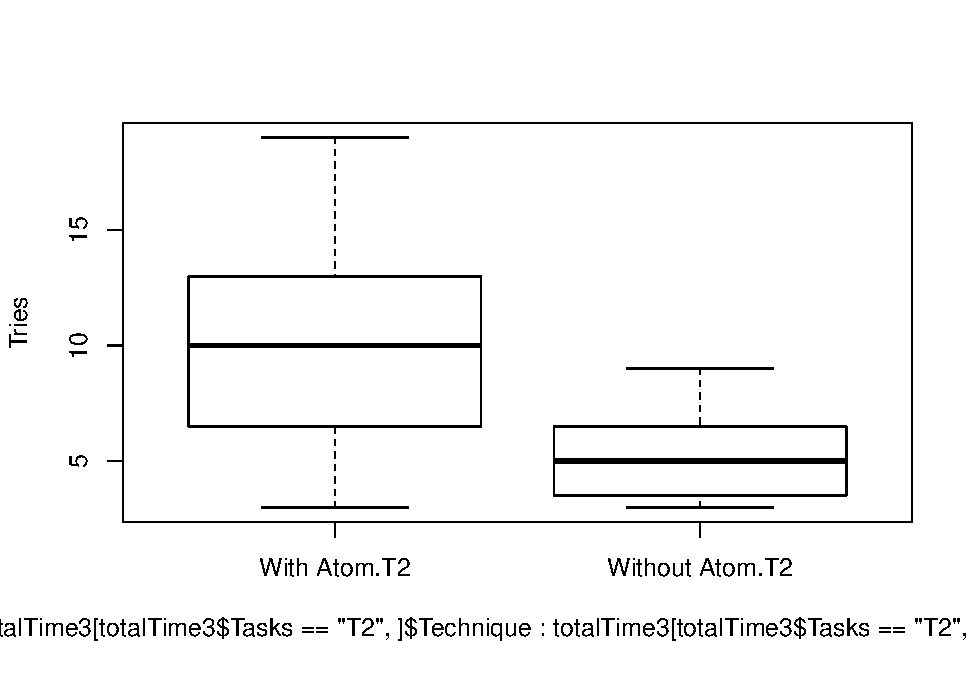
\includegraphics{main_files/figure-latex/unnamed-chunk-31-1.pdf}

\begin{Shaded}
\begin{Highlighting}[]
\NormalTok{totalTrials <-}\StringTok{ }\KeywordTok{sqldf}\NormalTok{(}\StringTok{"select Replica, Id, SetOfTasks,}
\StringTok{                      Technique, sum(Trials) as Trials}
\StringTok{                      from ccwocd where Tasks = 'AV2.1:CO2.1:DE2.1' or Tasks = 'AV2.2:CO2.2:DE2.2'}
\StringTok{                      group by Replica, Id,SetOfTasks, Technique"}\NormalTok{)}

\NormalTok{totalTrials}\OperatorTok{$}\NormalTok{Trials <-}\KeywordTok{ifelse}\NormalTok{(totalTrials}\OperatorTok{$}\NormalTok{Trials }\OperatorTok{==}\StringTok{ }\DecValTok{0}\NormalTok{, }\DecValTok{1}\NormalTok{, totalTrials}\OperatorTok{$}\NormalTok{Trials)}
\NormalTok{totalTrials}\OperatorTok{$}\NormalTok{Trials <-}\StringTok{ }\KeywordTok{with}\NormalTok{(totalTrials, }\KeywordTok{log2}\NormalTok{(Trials))}
\end{Highlighting}
\end{Shaded}

\begin{Shaded}
\begin{Highlighting}[]
\NormalTok{totalTrials}\OperatorTok{$}\NormalTok{Replica =}\StringTok{ }\KeywordTok{as.factor}\NormalTok{(totalTrials}\OperatorTok{$}\NormalTok{Replica)}
\NormalTok{totalTrials}\OperatorTok{$}\NormalTok{Id =}\StringTok{ }\KeywordTok{as.factor}\NormalTok{(totalTrials}\OperatorTok{$}\NormalTok{Id)}
\NormalTok{totalTrials}\OperatorTok{$}\NormalTok{SetOfTasks =}\StringTok{ }\KeywordTok{as.factor}\NormalTok{(totalTrials}\OperatorTok{$}\NormalTok{SetOfTasks}\OperatorTok{:}\NormalTok{totalTime}\OperatorTok{$}\NormalTok{Id)}
\NormalTok{totalTrials}\OperatorTok{$}\NormalTok{Technique =}\StringTok{ }\KeywordTok{as.factor}\NormalTok{(totalTrials}\OperatorTok{$}\NormalTok{Technique)}
\end{Highlighting}
\end{Shaded}

\begin{Shaded}
\begin{Highlighting}[]
\KeywordTok{summary}\NormalTok{(}\KeywordTok{aov}\NormalTok{(Trials }\OperatorTok{~}\StringTok{ }\NormalTok{Technique, }\DataTypeTok{data=}\NormalTok{totalTrials))}
\end{Highlighting}
\end{Shaded}

\begin{verbatim}
##             Df Sum Sq Mean Sq F value Pr(>F)  
## Technique    1  4.852   4.852   6.608 0.0158 *
## Residuals   28 20.560   0.734                 
## ---
## Signif. codes:  0 '***' 0.001 '**' 0.01 '*' 0.05 '.' 0.1 ' ' 1
\end{verbatim}

\begin{Shaded}
\begin{Highlighting}[]
\NormalTok{totalTrials.gvlma =}\StringTok{ }\KeywordTok{gvlma}\NormalTok{(}\KeywordTok{lm}\NormalTok{(Trials }\OperatorTok{~}\StringTok{ }\NormalTok{Technique, }\DataTypeTok{data=}\NormalTok{totalTrials))}
\KeywordTok{summary}\NormalTok{(totalTrials.gvlma)}
\end{Highlighting}
\end{Shaded}

\begin{verbatim}
## 
## Call:
## lm(formula = Trials ~ Technique, data = totalTrials)
## 
## Residuals:
##      Min       1Q   Median       3Q      Max 
## -1.62191 -0.56706 -0.08059  0.39815  2.18244 
## 
## Coefficients:
##                       Estimate Std. Error t value Pr(>|t|)    
## (Intercept)             3.2069     0.2213  14.494 1.53e-14 ***
## TechniqueWithout Atom  -0.8044     0.3129  -2.571   0.0158 *  
## ---
## Signif. codes:  0 '***' 0.001 '**' 0.01 '*' 0.05 '.' 0.1 ' ' 1
## 
## Residual standard error: 0.8569 on 28 degrees of freedom
## Multiple R-squared:  0.1909, Adjusted R-squared:  0.162 
## F-statistic: 6.608 on 1 and 28 DF,  p-value: 0.01576
## 
## 
## ASSESSMENT OF THE LINEAR MODEL ASSUMPTIONS
## USING THE GLOBAL TEST ON 4 DEGREES-OF-FREEDOM:
## Level of Significance =  0.05 
## 
## Call:
##  gvlma(x = lm(Trials ~ Technique, data = totalTrials)) 
## 
##                        Value p-value                Decision
## Global Stat        1.636e+00  0.8023 Assumptions acceptable.
## Skewness           1.544e+00  0.2140 Assumptions acceptable.
## Kurtosis           7.535e-02  0.7837 Assumptions acceptable.
## Link Function      7.228e-15  1.0000 Assumptions acceptable.
## Heteroscedasticity 1.623e-02  0.8986 Assumptions acceptable.
\end{verbatim}

\begin{Shaded}
\begin{Highlighting}[]
\KeywordTok{summary}\NormalTok{(}\KeywordTok{aov}\NormalTok{(Trials }\OperatorTok{~}\StringTok{ }\NormalTok{Technique, }\DataTypeTok{data=}\NormalTok{totalTrials))}
\end{Highlighting}
\end{Shaded}

\begin{verbatim}
##             Df Sum Sq Mean Sq F value Pr(>F)  
## Technique    1  4.852   4.852   6.608 0.0158 *
## Residuals   28 20.560   0.734                 
## ---
## Signif. codes:  0 '***' 0.001 '**' 0.01 '*' 0.05 '.' 0.1 ' ' 1
\end{verbatim}

\begin{Shaded}
\begin{Highlighting}[]
\NormalTok{ss =}\StringTok{ }\KeywordTok{summary}\NormalTok{(}\KeywordTok{aov}\NormalTok{(Trials }\OperatorTok{~}\StringTok{ }\NormalTok{Technique, }\DataTypeTok{data=}\NormalTok{totalTrials))[[}\DecValTok{1}\NormalTok{]]}\OperatorTok{$}\StringTok{"Sum Sq"}
\NormalTok{eta.sq =}\StringTok{ }\NormalTok{ss[}\DecValTok{1}\NormalTok{]}\OperatorTok{/}\NormalTok{(ss[}\DecValTok{1}\NormalTok{] }\OperatorTok{+}\StringTok{ }\NormalTok{ss[}\DecValTok{2}\NormalTok{])}
\KeywordTok{print}\NormalTok{(}\KeywordTok{paste0}\NormalTok{(}\StringTok{"The eta-squared is "}\NormalTok{,}\KeywordTok{toString}\NormalTok{(}\KeywordTok{round}\NormalTok{(eta.sq,}\DecValTok{3}\NormalTok{))))}
\end{Highlighting}
\end{Shaded}

\begin{verbatim}
## [1] "The eta-squared is 0.191"
\end{verbatim}

\begin{Shaded}
\begin{Highlighting}[]
\NormalTok{q <-}\StringTok{ }\KeywordTok{TukeyHSD}\NormalTok{(}\KeywordTok{aov}\NormalTok{(Trials}\OperatorTok{~}\NormalTok{Technique, }\DataTypeTok{data=}\NormalTok{totalTrials))}
\NormalTok{q}
\end{Highlighting}
\end{Shaded}

\begin{verbatim}
##   Tukey multiple comparisons of means
##     95% family-wise confidence level
## 
## Fit: aov(formula = Trials ~ Technique, data = totalTrials)
## 
## $Technique
##                              diff       lwr        upr     p adj
## Without Atom-With Atom -0.8043511 -1.445296 -0.1634066 0.0157578
\end{verbatim}

\begin{Shaded}
\begin{Highlighting}[]
\NormalTok{slices <-}\StringTok{ }\KeywordTok{c}\NormalTok{(}\DecValTok{67}\NormalTok{, }\DecValTok{33}\NormalTok{) }
\NormalTok{lbls <-}\StringTok{ }\KeywordTok{c}\NormalTok{(}\StringTok{"Perfectiva"}\NormalTok{, }\StringTok{"Não Perfectiva"}\NormalTok{)}
\NormalTok{pct <-}\StringTok{ }\KeywordTok{round}\NormalTok{(slices}\OperatorTok{/}\KeywordTok{sum}\NormalTok{(slices)}\OperatorTok{*}\DecValTok{100}\NormalTok{)}
\NormalTok{lbls <-}\StringTok{ }\KeywordTok{paste}\NormalTok{(lbls, pct) }\CommentTok{# add percents to labels }
\NormalTok{lbls <-}\StringTok{ }\KeywordTok{paste}\NormalTok{(lbls,}\StringTok{"%"}\NormalTok{,}\DataTypeTok{sep=}\StringTok{""}\NormalTok{) }\CommentTok{# ad % to labels }
\KeywordTok{pie}\NormalTok{(slices,}\DataTypeTok{labels =}\NormalTok{ lbls, }\DataTypeTok{col=}\KeywordTok{rainbow}\NormalTok{(}\KeywordTok{length}\NormalTok{(lbls))}
\NormalTok{  )}
\end{Highlighting}
\end{Shaded}

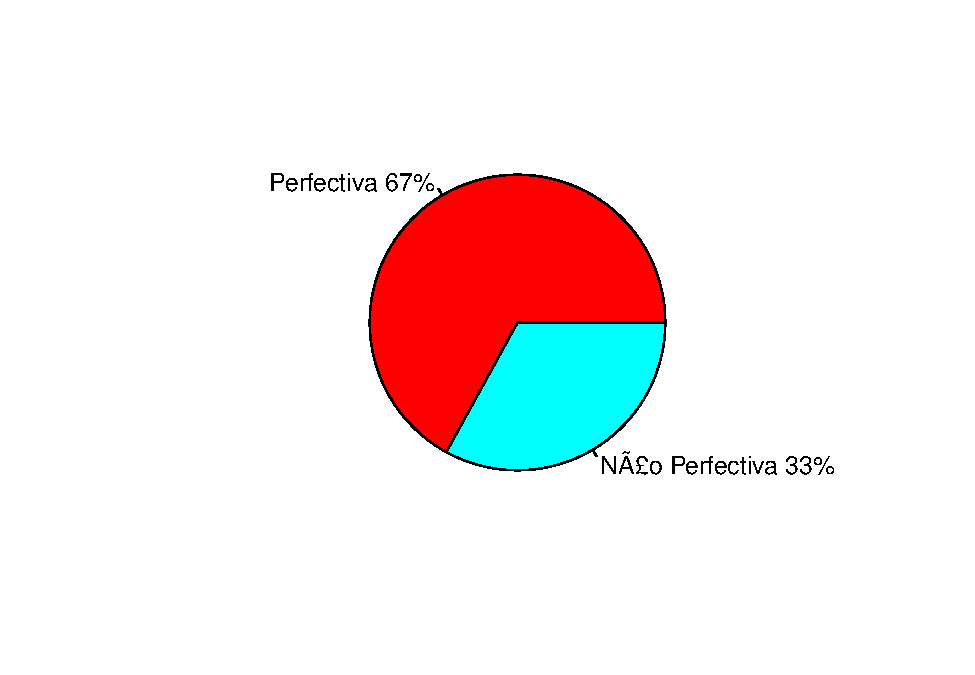
\includegraphics{main_files/figure-latex/unnamed-chunk-38-1.pdf}


\end{document}
